\chapter{Data Preprocessing and Feature Engineering}
\label{chap6}

So far, the data collected are:

\begin{itemize}
    \item the frames that were captured during the finalized render sequences, encapsulating the luminance reflected by the surfaces and reaching the SCC,
    \item the absolute rotation (in roll, pitch and yaw) and cartesian coordinates of the SCC inside the simulation, recorded for each frame captured,
    \item the absolute rotation (in roll, pitch and yaw) of the sun, recorded for each render sequence, with the roll angle being set equal to the the SZA throughout the experiment,
    \item the readings and absolute cartesian coordinates of the light meters and,
    \item the assigned GRVI value of the material applied to each area of the field.
\end{itemize}

Considering that, the algorithms selected to be trained for correcting the perceived GRVI values are mainly shallow Multi-Level Perceptrons and ensemble ML methods, this data should be structured in a way interpretable for them. The processed I followed for achieving that is described in this chapter.

\section{Data Preprocessing}
\label{dp}

Considering the nature of the ML models that were elected as ideal for this application, transforming the collected information into tabular data - data structured into rows and columns, much similar to a spreadsheet - seemed fairly intuitive. Ensemble methods in particular have historically performed strongly in classification and regression tasks with tabular data as inputs \cite{tabdata-gen}, while specially tuned NN architectures have begun to emerge for these applications \cite{tabnet, tabdata-nn}. 


In this study, each row corresponds to an area-of-interest extracted from the frames captured during the render sequences, while each column provides the information necessary for each area-of-interest. As a reminder, the areas-of-interest for which the GRVI values were calculated are twenty adjacent square regions arranged horizontally across the image, with their common vertical position being the vertical center of the frame (Figure~\ref{aoi}). Before any kind of feature engineering was performed, the data I decided to include as inputs for the trained algorithms were (along with their column names when stored in .csv files):

\begin{itemize}
    \item the average perceived GRVI value of the area-of-interest ($grviIn$),
    \item the average red and green reflectance of the area-of-interest ($meanRefR$ \& $meanRefG$),
    \item measured illuminance for the red and green bands, either unique to the sample or the render sequence (more on that later) ($illumR$ \& $illumG$),
    \item index of the area-of-interest within the frame it was extracted from (bolckIdx),
    \item roll, pitch and yaw of the sun ($sunRoll$, $sunPitch$ \& $sunYaw$),
    \item roll, pitch and yaw of the SCC ($camRoll$, $camPitch$, \& $camYaw$), and
    \item the target value ($grviOut$)
\end{itemize}

Other information that could be included in the inputs was the average red and green luminance of the area-of-interest, but I avoided it since, considering that the final objective is deployment on an edge device, redundancy would noticeably increase computational overhead. For the same reason, several of these features were removed later on. From the information mentioned in the introduction of this chapter, the SCC's location data were not included in order to avoid spoonfeeding the model, considering that it should perform while being agnostic to location. The light meters' location data were also not used as features since they did not provide meaningful information. However, both SCC's and light meters' coordinates were used during data preprocessing

Most of the aforementioned features were directly available for being structured into the desired format. The data associated with the measured reflectance of the studied surfaces and, consequently, GRVI, though, had to be drawn out from the captured frames and calculated using other contributing metrics.

\subsection{Calculating Input Reflectance and GRVI}

As mentioned in Section~\ref{photom-q-meas}, the reflectance of a surface is calculated using the reflectance formula for Lambertian surfaces:

\begin{equation}
    \rho_b = \frac{L_b \times \pi}{E_b}\,,
    \label{lambertian1}
\end{equation}

with $\rho_b, L_b$ and $E_b$ being the reflectance, luminance, and illuminance per band, respectively. Therefore, the calculation of reflectance can be separated into three stages: extracting luminance per band for the surfaces presented in the area-of-interest, acquiring the illuminance reaching these surfaces and eventually performing the calculation. 

To retain the luminance of the areas-of-interest, the captured images had to be read sequentially, maintaining the green- and red-channel values of the selected points in the process. The images were previously organized in a way that each of them belonging to a render sequence was stored in the same folder and indexed relative to the other images in the same sequence, based on the order they have been rendered. All the folders corresponding to render sequences were stored under a shared "home" folder. I developed a Python script that, given this "home" folder, it serially opens the folders existing within it, traversing through the frames they contain. Eventually, for each frame read, the script isolates the $20$ areas-of-interest and stores their red and green channels as NumPy arrays.

!!! present here folder architecture!!!

In order to use these arrays to calculate GRVI, the illuminance for each area-of-interest should also be known. As mentioned throughout this study, there were mainly three ways used for acquiring the illuminance of the scene: single stationary light meter, multiple light meters measuring the illuminance of the points included in the camera's field of view and single light meter attached to the same rig as the camera, measuring the illuminance near the camera. I used the first method in cases where there were no obstacles between the light source and the field's canopy. The light meter reading remained the same during each render sequence. I stored the measured value of each sequence in .txt files within the corresponding folder. This way, it was simple to use the same script that traverses through the captured frames to parse the illuminance values and, during calculations, use the appropriate one for each render sequence.

The second and third ways of measuring illuminance aimed to address the lack of robustness to illumination variability of the first. In the multiple light meter case, the readings and position of each sensor were stored in separate .txt files, again, residing within the corresponding render sequence folder. With five sensors deployed in the scene, there were five files created for each illumination scenario. Each row of the files refers to the respectively indexed frame, and contains information regarding four of its areas-of-interest. Consequently, the information found in all rows with the same index across the five files provides complete complete context for all the areas-of-interest of one frame. During the GRVI calculation, the Python script parses the light meter files and matches the readings with the appropriate frames based on their row index. For the single sensor approach, the illuminance readings corresponding to the central four areas-of-interest are used, captured during the multiple sensor approach. During GRVI, specifically while parsing the readings file, I shifted the readings to align the position of the camera and the sensor, matching each frame with the readings originally targeted for the previous.  The first frame and last sensor readings are discarded.

With the luminance of each area-of-interest represented as an array of pixel values and the corresponding illuminance measurements parsed, the next step was to calculate the red- and green-band reflectance of the depicted surfaces using Equation~\ref{lambertian1}. Both $\pi$ and the illuminance value were broadcast for multiplication and division with the luminance array. The red-band illuminance is used along with the red-band luminance, with the same process followed for the green-band measurements. The results are two arrays, each cell of which represents the reflectance of a tiny part of the captured surfaces in the respective bands. The average values of red- and green-band reflectance arrays were used as two of the features of the dataset.

Finally, the script calculates GRVI for every frame's areas-of-interest. Again, there are two possible approaches for calculating the average GRVI value of each cropped part of the frame. The first uses the calculated means of the reflectance arrays to output a single GRVI value (Equation~\ref{avgRefGrvi}). This method provided stable values with limited outliers, making it ideal for calculating the reference GRVI values using the frames collected under diffuse lighting conditions. The second approach was calculating GRVI using directly the red and green reflectance arrays (Equation~\ref{avgGRVI}). This results in a GRVI array containing a value for every pixel of the given area-of-interest. The mean of the array is then calculated and used as an input feature. The values produced using this method were particularly unstable, with multiple outliers, including measurements with absolute values greater than $1$, which is abnormal for a normalized index such as GRVI, whose values are capped in the $\begin{bmatrix}
    -1, & 1
\end{bmatrix}$ space. 

\begin{equation}
    GRVI = \frac{avg(\begin{bmatrix}RefG\end{bmatrix}) - avg(\begin{bmatrix}RefR\end{bmatrix})}{avg(\begin{bmatrix}RefG\end{bmatrix}) + avg(\begin{bmatrix}RefR\end{bmatrix})}
    \label{avgRefGrvi}
\end{equation}

\begin{equation}
    GRVI = avg(\begin{bmatrix}GRVImat\end{bmatrix}) = avg(\frac{\begin{bmatrix}RefG\end{bmatrix} - \begin{bmatrix}RefR\end{bmatrix}}{\begin{bmatrix}RefG\end{bmatrix} + \begin{bmatrix}RefR\end{bmatrix}})
    \label{avgGRVI}
\end{equation}

Both GRVI calculation methods display advantages and disadvantages when their output is used as input feature. The first provides stable values, but since the mean reflectance values in the two bands are already provided to the models, GRVI calculated using them is expected to provide limited additional information. The second method on the other hand, despite producing inaccurate values, could complement the context provided by the rest of the features. When it comes to the output GRVI, only the first method was used. As for the inputs, I created datasets using both methods, exploring the impact of each of them to the models' performance. 

The complete GRVI calculation pipeline is illustrated in Figure~\ref{PLaceHolder!!!!}.

\subsection{Create Datasets' Target Values}

With all the input features ready, the remaining task for the development of the datasets was the preparation of the target values. I created two kinds of datasets, regarding the type of the values the models were trained to approximate.

In the first kind, the target values were calculated using the perceived red- and green-band reflectance values, as they were perceived in the digital twin under diffuse lighting conditions. Using the frames rendered during the two sequences I performed for diffuse lighting conditions - one following the data-collection spline from its beginning to its end and one following the opposite route - and the version of the GRVI calculation pipeline described above, where the averages of the reflectance matrices are used, the result was two single column arrays, stored as .csv files. Each row represents the target GRVI value for each area-of-interest.

In the second, the target values were the ones I assigned to each material used. The crucial step in this case was identifying the parts of the field depicted in each frame, making possible the mapping of each area-of-interest with its inherent GRVI value. To perform this task, I developed another script that, using the camera coordinates during each frame-capture and given that the field is separated in $1.9m \times 1.9m$ parts, calculates which part (or parts) is depicted, and therefore which inherent material is present. Considering that, when a frame is captured in landscape orientation, a wide area is included in the final rendered image, there is always the possibility that more than one parts of the field are depicted. It was important that the script took account of this case and map different inherent GRVI values to each frame's areas-of-interest when needed. 

To do so, I had to estimate how the horizontal length of each area-of-interest maps into the digital twin. With the simplifying assumption that the SCC's simulated lens is not curved, I approximated the distance between the edges of leftmost and rightmost areas-of-interest to be $680$ centimeters within the simulation. Assuming also that that the counterpart of each area-of-interest in the digital twin has the same length as the others, the script is able to identify the bounds of each area-of-interest within the simulation and decide which part of the field each of them depicts, mapping eventually each of them to an inherent GRVI value. The pipeline for this process if illustrated in Figure~\ref{PlaceHolder!!!}. The results for both the beginning-to-end route and the opposite were saved in single column .csv files.

\subsection{Dataset Creation}
With the preparation of the average red- and green-band reflectance values and the perceived GRVI value for each frame's areas-of-interest, and both the labels based on measured and assigned GRVI values, all the data necessary for the models' training were available. The last step for creating the initial versions of the datasets was gathering all the data scattered across different files and folders and combining them in an easily interpretable by algorithms format.

The initial datasets I had decided to develop are:
\begin{itemize}
    \item Using as labels GRVI measurements under diffuse lighting conditions:
    \begin{enumerate}
        \item field without trees,
        \item field with trees - light meters ahead of camera,
        \item field with trees - light meters close to camera,
        \item 1. and 2. combined,
        \item 1. and 3. combined.
    \end{enumerate}
    \item Using as labels inherent GRVI values:
        \begin{enumerate}
        \item field without trees,
        \item field with trees - light meters ahead of camera,
        \item field with trees - light meters close to camera,
        \item 1. and 2. combined,
        \item 1. and 3. combined.
    \end{enumerate}
\end{itemize}

In all of the input samples, the sky is clear and the illumination scenarios are the ones presented in Table~\ref{ilmsce} (except GT conditions). The input features in all of the datasets are the ones presented in the beginning of section~\ref{dp}.

The selected method of storing the datasets was in .csv files. The Python script used for traversing the image folders and calculating the GRVI per area-of-interest was modified to handle the structuring of the data in this format. Specifically, every time the script accesses a render sequence folder, it creates an empty Pandas DataFrame object. As the program proceeds to open the contained frames and calculate the average perceived GRVI value for each of their areas-of-interest, the result, along with the rest of the features associated with it (mean calculated reflectance, index within frame, illuminance, sun and camera rotation) are stored as rows in the DataFrame. By the time all the images of a render sequence folder have been accessed, the DataFrame is stored on the hard drive as a .csv file containing information regarding only this sequence. I decided to first save the data for each render sequence separately because handling missing data and eventually matching inputs with target values was found to be simpler when working on a single sequence's data.

Post the creation of the files for the separate files, the remaining steps were adding the target value's column and combining the separate files into a complete dataset. I had already organized the target values in single column .csv files, correctly aligned with the indexing of the samples contained in the created files. That means that, by the time I developed a script that adds labels to the input features and combines them to a single dataset, adding the labels was as simple as assigning to the "grviOut" column of the DataFrame the target values column. I had developed the script with options on whether to traverse folders of scenarios with trees, without trees or both, and using or not the assigned GRVI values as ground truth. Eventually, all ten of the initially planned datasets were created.

\subsection{Alternative Datasets}

The initial datasets were meant to be used for training algorithms that consist of a single model. These architectures were expected to address all possible sources of error involved during the GRVI calculations, with the minimum degree of error possible. Another method I experimented with to minimize this error even further was training and combining different models designed to handle different sources of error into one hierarchical architecture, creating essentially a mixture of experts. This process required modifying the already existing datasets to be compatible with the training pipelines of each of the models included in the final system.

\subsubsection{Dataset for Shadow Detection Model Training}

One of the architectures I experimented with was a hard-gated mixture of experts, aiming to handle data acquired from shaded scenes differently than the rest. The key mechanism for choosing the appropriate model every time an input is given is a classifier responsible for identifying wether the shadow of a tree was present when a frame was collected. 

To train this classifier, a second version of the datasets that include trees had to be developed. Specifically, the originals' target values were the materials' ground truth GRVI values. For this task, the target values have to be binary labels, indicating wether the studied area-of-interest depicts shaded parts of the field not. Upon inspecting the data collected during the different render sequences, the common characteristic I found amongst all information captured while shadows were present was naturally the particularly low illuminance values, as they were measured by the light meters. This is caused due to the interference of the trees between the light meters and the light source.

For the datasets constructed using directly the collected data, identifying the images depicting shaded parts was as simple as comparing the associated measured green-band illuminance with a loosely defined threshold. This is possible since the lowest assigned green-band illuminance, featured in Table~\ref{ilmsce}, is $200$, while the illuminance measured in shaded parts is typically a single digit number, regardless the light source's intensity. By performing this comparison for all the samples, I added an additional column to these datasets, indicating whether there was a shadow present in the scene when the frame was taken, and whether the particular area-of-interest was within the occluded area.

Arguably, the addition of shadow-presence-indicating labels and training of ML models for the classification of shadows for these datasets is redundant. That said, it was mainly performed for later transferring these labels to the datasets constructed by shifting the central light meter's readings, simulating that a single light meter was mounted close to the camera. In these cases, the identification of shadows relies on more complex patterns within the data, since the light meter's readings could differ from the actual illuminance values near the studied area of difference. Eventually, I was able to directly transfer the labels calculated for the areas-of-interest from the dataset with the accurate light meters' readings to the rest of the datasets where shadows were present, since they are invariant to the light meters' positioning.

The result was the four original datasets which include data derived from shaded scenes, with an extra binary indicator. This indicator signifies whether the respective area of interest depicts a part of the scene that is occluded.

\section{Feature Engineering}
\label{feature-eng}

The initially created datasets aimed to provide a first idea of what is the predictive performance of the proposed ML models for this particular task. The next step was achieving a satisfying balance between predictive performance and computational efficiency. This task can be achieved with feature engineering. By performing feature engineering, it was possible to both reduce the dimensions of the original dataset and make the provided information more easily interpretable to the models.

This section aims to present the possible different feature engineering methods that I considered to employ for creating different version of the dataset, with the final goal being the aforementioned accuracy-compactness balance. The impact of each of these methods on these examined factors is discussed in the !!!! chapter !!!!.


\subsection{Dimensionality Reduction}

%% say stuff!!


\subsubsection{Feature Selection}
\label{feature-sel}

A common feature engineering practice is reducing dimensionality by dropping unimportant input attributes. An instance of such is low-variance features, being features that hardly change throughout the dataset. Another example is features that are strongly correlated with others. Finally, it is possible that one of the inputs simply does not provide any noticeable impact on the output's estimation.

When it comes to low-variance features, several can be directly identified by a quick dataset inspection. Specifically, $sunRoll$ and $camRoll$ remain the same and equal to $180$ and $0$, respectively, throughout all the examples, therefore were found safe to be removed. $camPitch$ was also expected to remain set to $-20$, but throughout the examples, the value seems to have subtle fluctuations. Therefore, I considered it better to run feature importance tests and validate its insignificance before dropping it.

Regarding correlated features, I found the Pearson Correlation Coefficient to be a fairly informative tool for identifying linear relationships between the features. I used it to construct correlation heatmaps for several of the previously mentioned versions of the dataset. However, the results among all tested iterations were expectedly close. One of the produced correlation maps is presented in Figure~\ref{correlation-hm}. The features $sunRoll$ and $camRoll$ remain constant throughout the dataset and therefore no coefficients were calculated between them and the other features. $illumG$ and $illumR$ are used for the calculations of $meanRefG$ and $meanRefR$, respectively, and therefore it is natural that they are correlated. Furthermore, throughout the simulation, as illuminance for one band grew, it grew for the other band as well, explaining why there is a strong relationship between them. It can also be seen that the perceived reflectance of each band follows the trend of the other band, while none of them is strongly correlated to $grviIn$. This is the case because. Lastly, $grivOut$ does not appear to be linearly related to any other feature. In a vacuum, that could be concerning, since $grviOut$ is expected to behave similarly to $grviIn$. That said, due to the infulence of directional light and shadows, $grviIn$'s values are expected to be unstable. Overall, it is seen later on that the models are able to learn the relationship between input features and the target values, implying the existence of non-linear relationships between them.

\begin{figure} [htb]
    \centering
    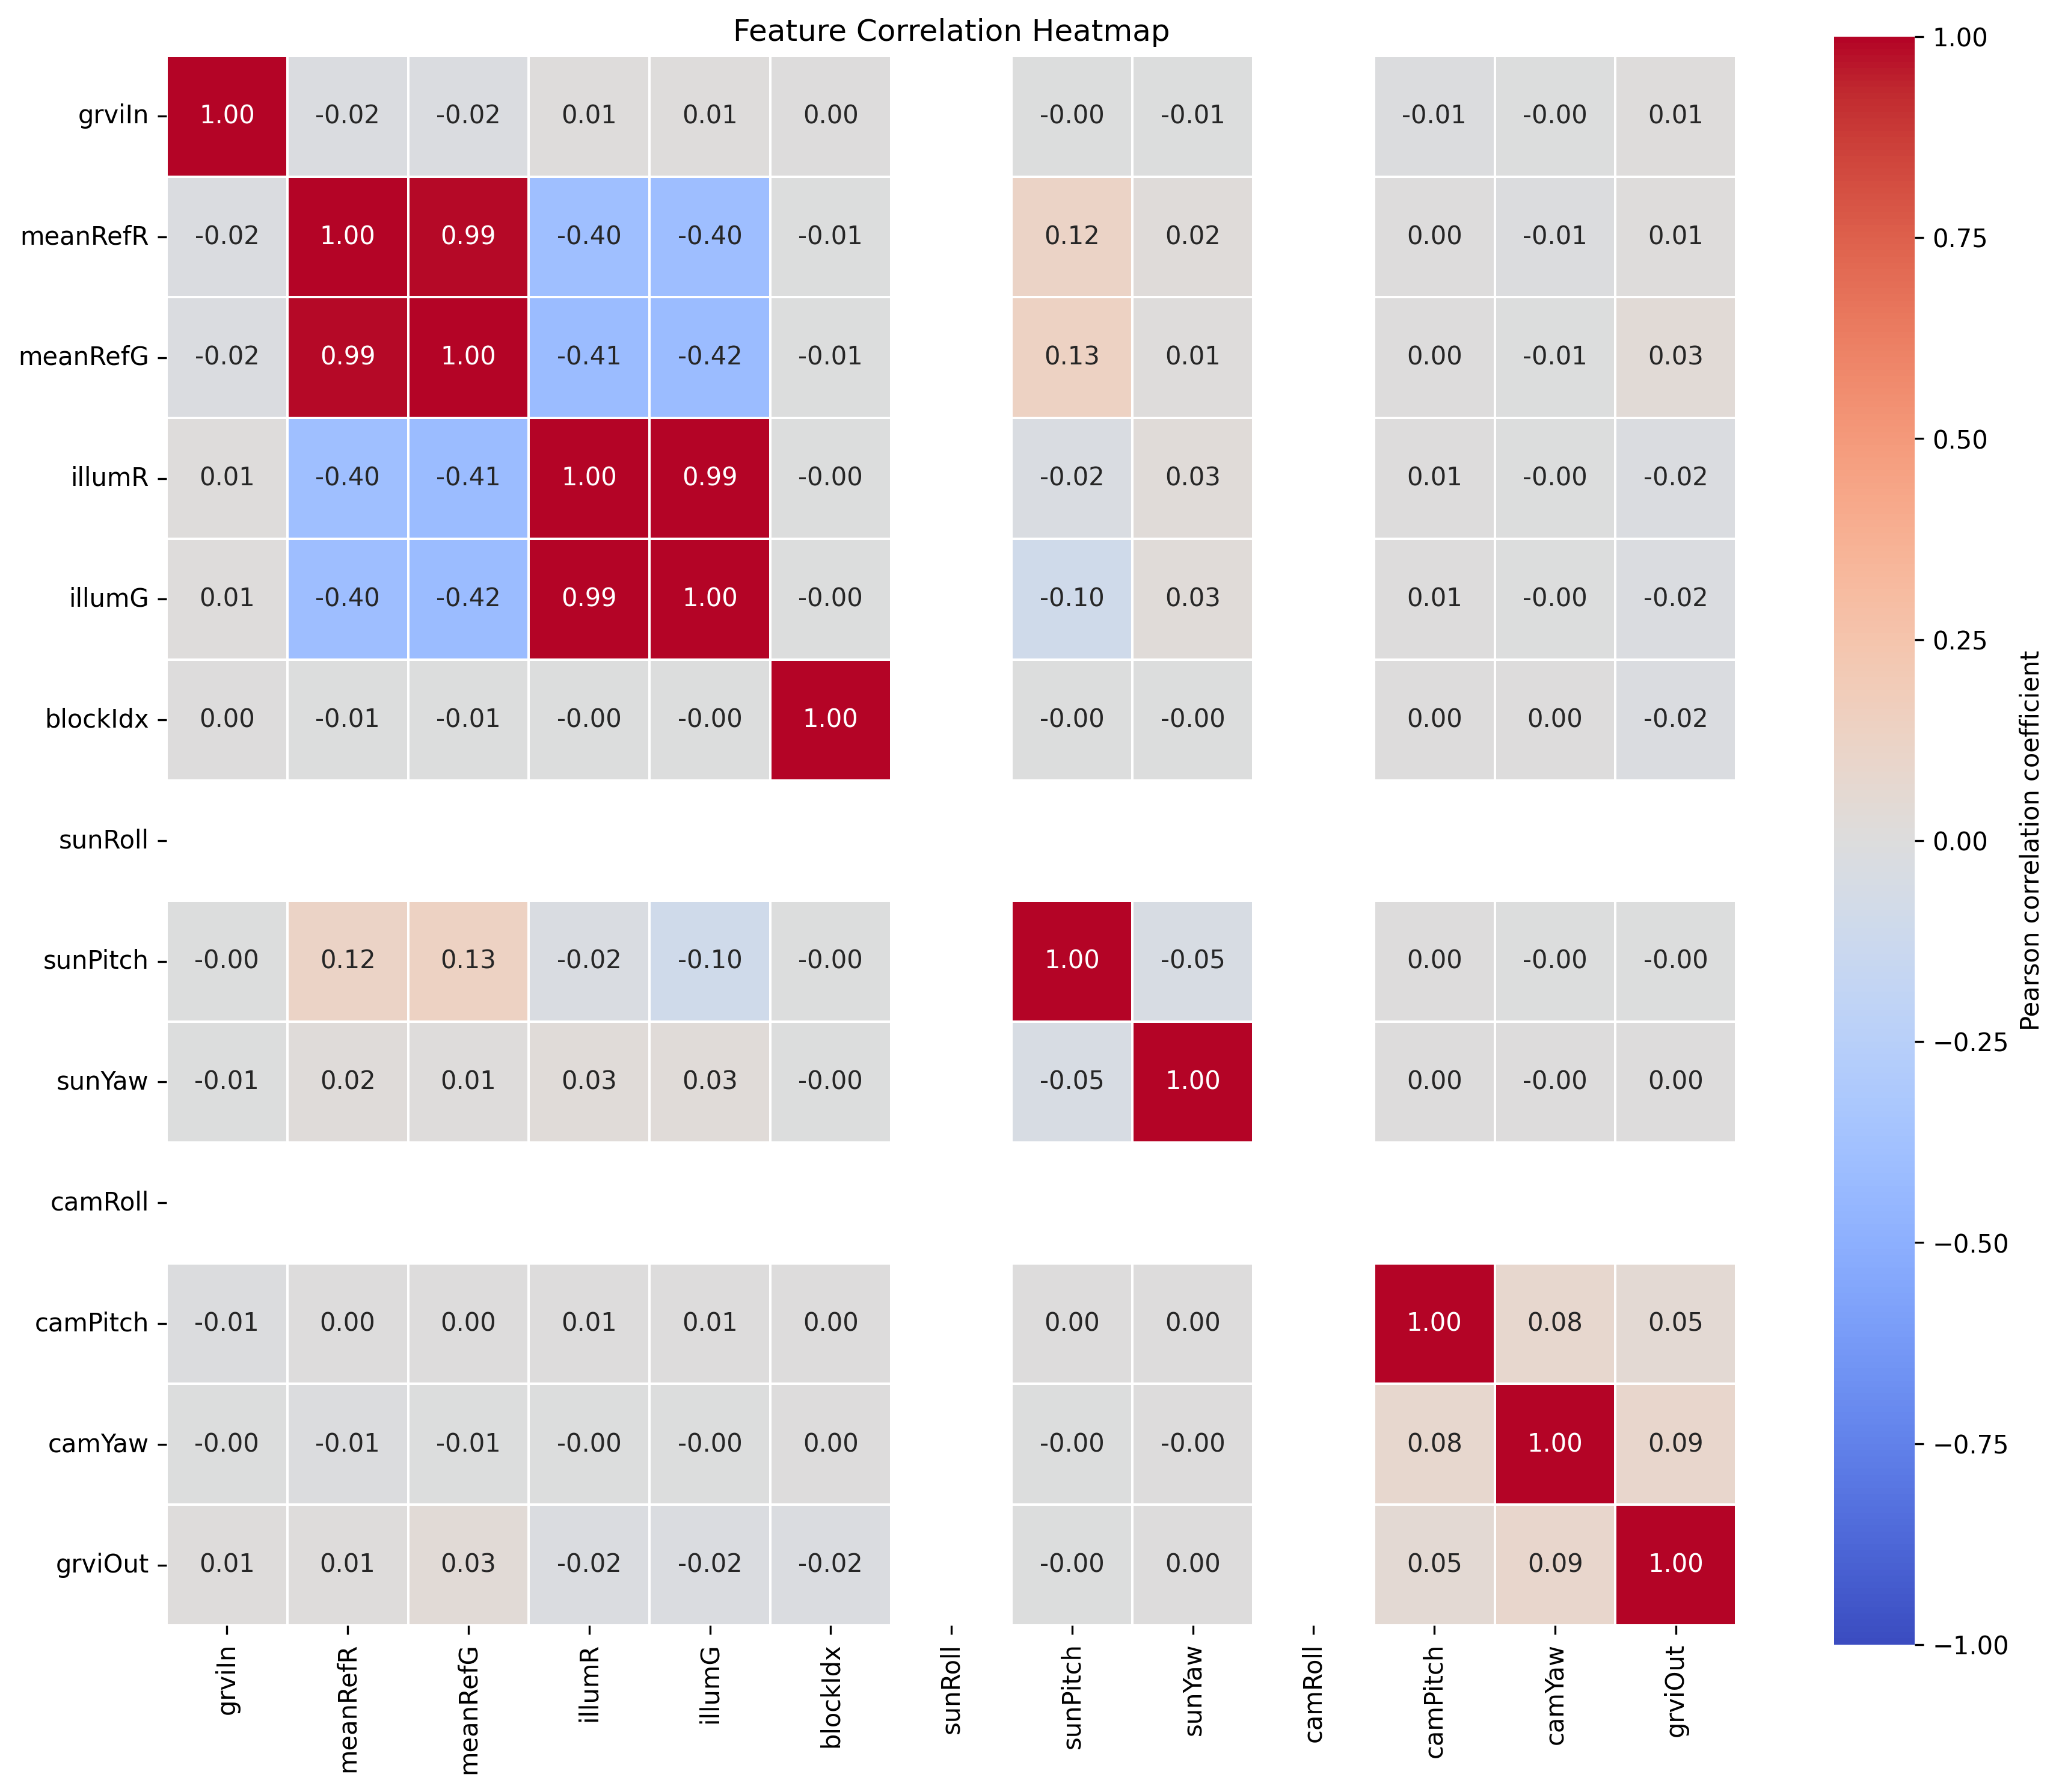
\includegraphics[width=1\linewidth]{images/correlation_trees-dl-aoi.png}
    \caption{Correlation heatmap presenting the Pearson Correlation Coefficient calculated between all the features of the dataset.}
    \label{correlation-hm}
\end{figure}


Another way to identify which features could be safely dropped without major loss in predictive performance is by determining the importance of each feature. All of the frameworks used for their implementations of classical ML models provide tools for calculating feature importance, such as permutation feature importance, impurity-based importance, etc. Since these methods are model-dependent, they are discussed later on, after the models' implementations, in Section~\ref{pract-feature-eng}.

\subsubsection{Principal Component Analysis (PCA)}

Principal component analysis (PCA) aims to reduce the complexity of a given dataset by replacing its features with new, uncorrelated ones, named principal components, while attempting to retain as much useful information as possible. Mathematically, this means that the original data are projected to a lower dimensional subspace, in a way that variance of the projected data is maximized (as much as possible of the original variance is preserved) \cite{shlens2005pca}.

I experimented with PCA, aiming to determine weather it achieves dimensionality reduction more efficiently than the rest of the methods tested throughout this study. This included testing different amounts of principal components, seeking for a sweet-spot between low count of principal components and high predictive accuracy. The results are discussed in !!!!!!!!!.

\subsubsection{Substituting Sun's and SCC's Roll, Pitch and Yaw with a Single Number}

Among the attributes that were originally planned to be included in the datasets, there were a total of six regarding the sun-SCC geometry: the sun's and SCC's roll, pitch and yaw (RPY). Although some of them could be easily removed during the feature selection, it is possible to reduce all of them to a single feature, by replacing them with the relative azimuth angle between the sun and the SCC. 

To reduce the six RPY features, the first step was to convert these values into the corresponding rotation matrices of the two actors' unit vectors. For a given set of RPY angles, the rotation matrix is defined as \cite{rot-mat}:

\[ 
R = R_z(\mathrm{yaw})R_y(\mathrm{pitch})R_x(\mathrm{roll}),
\]


where

\[
R_z(\mathrm{yaw}) =
\begin{bmatrix}
\cos(\mathrm{yaw}) & -\sin(\mathrm{yaw}) & 0\\
\sin(\mathrm{yaw}) & \cos(\mathrm{yaw}) & 0\\
0 & 0 & 1
\end{bmatrix},
\]

\[
R_y(\mathrm{pitch}) =
\begin{bmatrix}
\cos(\mathrm{pitch}) & 0 & \sin(\mathrm{pitch})\\
0 & 1 & 0\\
-\sin(\mathrm{pitch}) & 0 & \cos(\mathrm{pitch})
\end{bmatrix},
\]

and

\[
R_x(\mathrm{roll}) =
\begin{bmatrix}
1 & 0 & 0\\
0 & \cos(\mathrm{roll}) & -\sin(\mathrm{roll})\\
0 & \sin(\mathrm{roll}) & \cos(\mathrm{roll})
\end{bmatrix}.
\]

Thus, separate rotation matrices \(R_c\) and \(R_s\) were calculated for the SCC and the Sun, respectively.

In Unreal Engine (UE), the \(x\)-axis represents the forward direction, while the \(y\)-axis represents the right direction. Therefore, the SCC's local forward and right directions can initially be represented by the unit vectors:

\[
\begin{bmatrix}1\\0\\0\end{bmatrix}
\quad\text{and}\quad
\begin{bmatrix}0\\1\\0\end{bmatrix}.
\]

These vectors were rotated using \(R_c\) so that they followed the actual orientation of the SCC. The resulting forward and right vectors were therefore calculated as:

\[
f_c = R_c
\begin{bmatrix}
1\\0\\0
\end{bmatrix},
\qquad
r_c = R_c
\begin{bmatrix}
0\\1\\0
\end{bmatrix}.
\]

Together, \(f_c\) and \(r_c\) define the SCC-relative plane onto which the sun's direction can be projected. 


For the sun, on the other hand, only the forward direction is required since its only used to determine the direction in which it is pointing. Its corresponding vector was obtained as:

\[
s = R_s
\begin{bmatrix}
1\\0\\0
\end{bmatrix}.
\]

In general, the angle between two arbitrary vectors \(a\) and \(b\) can be determined through their dot product, using \cite{wikipedia2025dot}:

\[
\theta =
\arccos\left(
\frac{a\cdot b}
{\lVert a\rVert\lVert b\rVert}
\right).
\]

In this case, \(f_c\), \(r_c\), and \(s\) are unit vectors and therefore have a magnitude of one. Consequently, the expression simplifies to:

\[
\theta = \arccos(a\cdot b).
\]

The dot product between the sun direction and the SCC forward direction consequently represents the cosine component of the relative angle,

\[
\frac{s\cdot f_c}
{\lVert s\rVert\lVert f_c\rVert}
=
\cos(\theta)
\quad\Rightarrow\quad
s\cdot f_c = \cos(\theta),
\]

while, since the SCC's right direction is perpendicular to its forward direction, the corresponding right component is:

\[
s\cdot r_c = \sin(\theta).
\]

These two components can then be combined using the two-argument arctangent function. In general \cite{wikipedia2025atan2}:

\[
\theta = \operatorname{atan2}(y,x),
\]

where

\[
x=r\cos(\theta),
\qquad
y=r\sin(\theta).
\]

Therefore, using the forward component as \(x\) and the right component as \(y\), the relative sun–SCC azimuth is obtained as

\begin{equation}
    \theta =
    \operatorname{atan2}
    \left(
    s\cdot r_c,\,
    s\cdot f_c
    \right)
\end{equation}


I later coded this sequence of operations into a Python script that, given a dataset including the sun's and SCC's RPY as input features, replaces the six rotation columns with a single relative azimuth angle column. The predictive and computational performance impacts of this change are discussed in !!!!!!!!!.

\subsection{Standard Scaling}
\label{standscale}

As demonstrated in Section~\ref{diffuse-aff-grvi}, the perceived GRVI values calculated using luminance and illuminance information under diffuse lighting conditions tend to be concentrated within a particularly narrow range, even after removing the removal of soil. While this characteristic is not inherently problematic, differences in the numerical scales of input features can disproportionately influence certain scale-sensitive ML algorithms, regardless of the features' actual predictive importance \cite{google_normalization}. In our case, while the average perceived GRVI values are within the range $\begin{bmatrix}0.059267, 0.184111\end{bmatrix}$, the illuminance values range between $0.253$ and $1467.124$. Tree-based methods, which were the primary architecture I experimented with in this work, are insensitive to feature scaling \cite{sklearn_feature_scaling}. However, other algorithms, particularly those relying on distance calculations, regularization, or gradient-based optimization, such as Ridge Regression, Lasso Regression, Support Vector Regression and Neural Networks, can be significantly affected by such differences.

A solution to the problems introduced by having features on different scales is bringing all features to a common scale. This eliminates disproportionate influence on the ouput, caused solely by a feature's magnitude. In this study, I used Scikit-learn's implementation of Z-score scaling, called Standard Scaling, to scale the data. Z-score scaling transforms each numerical feature so that it has mean equal to $0$ and standard deviation equal to $1$. As expected, the application of Standard Scaling to the datasets did not affect tree-based models, the impact on the rest of the models though was noticeable. Figure~\ref{ss-before-after} illustrates the feature values corresponding to the areas of interest of frames captured during one of the render sequences, before and after Standard Scaling.

\begin{figure}[htb]
    \centering
    
    \begin{subfigure}{0.48\linewidth}
        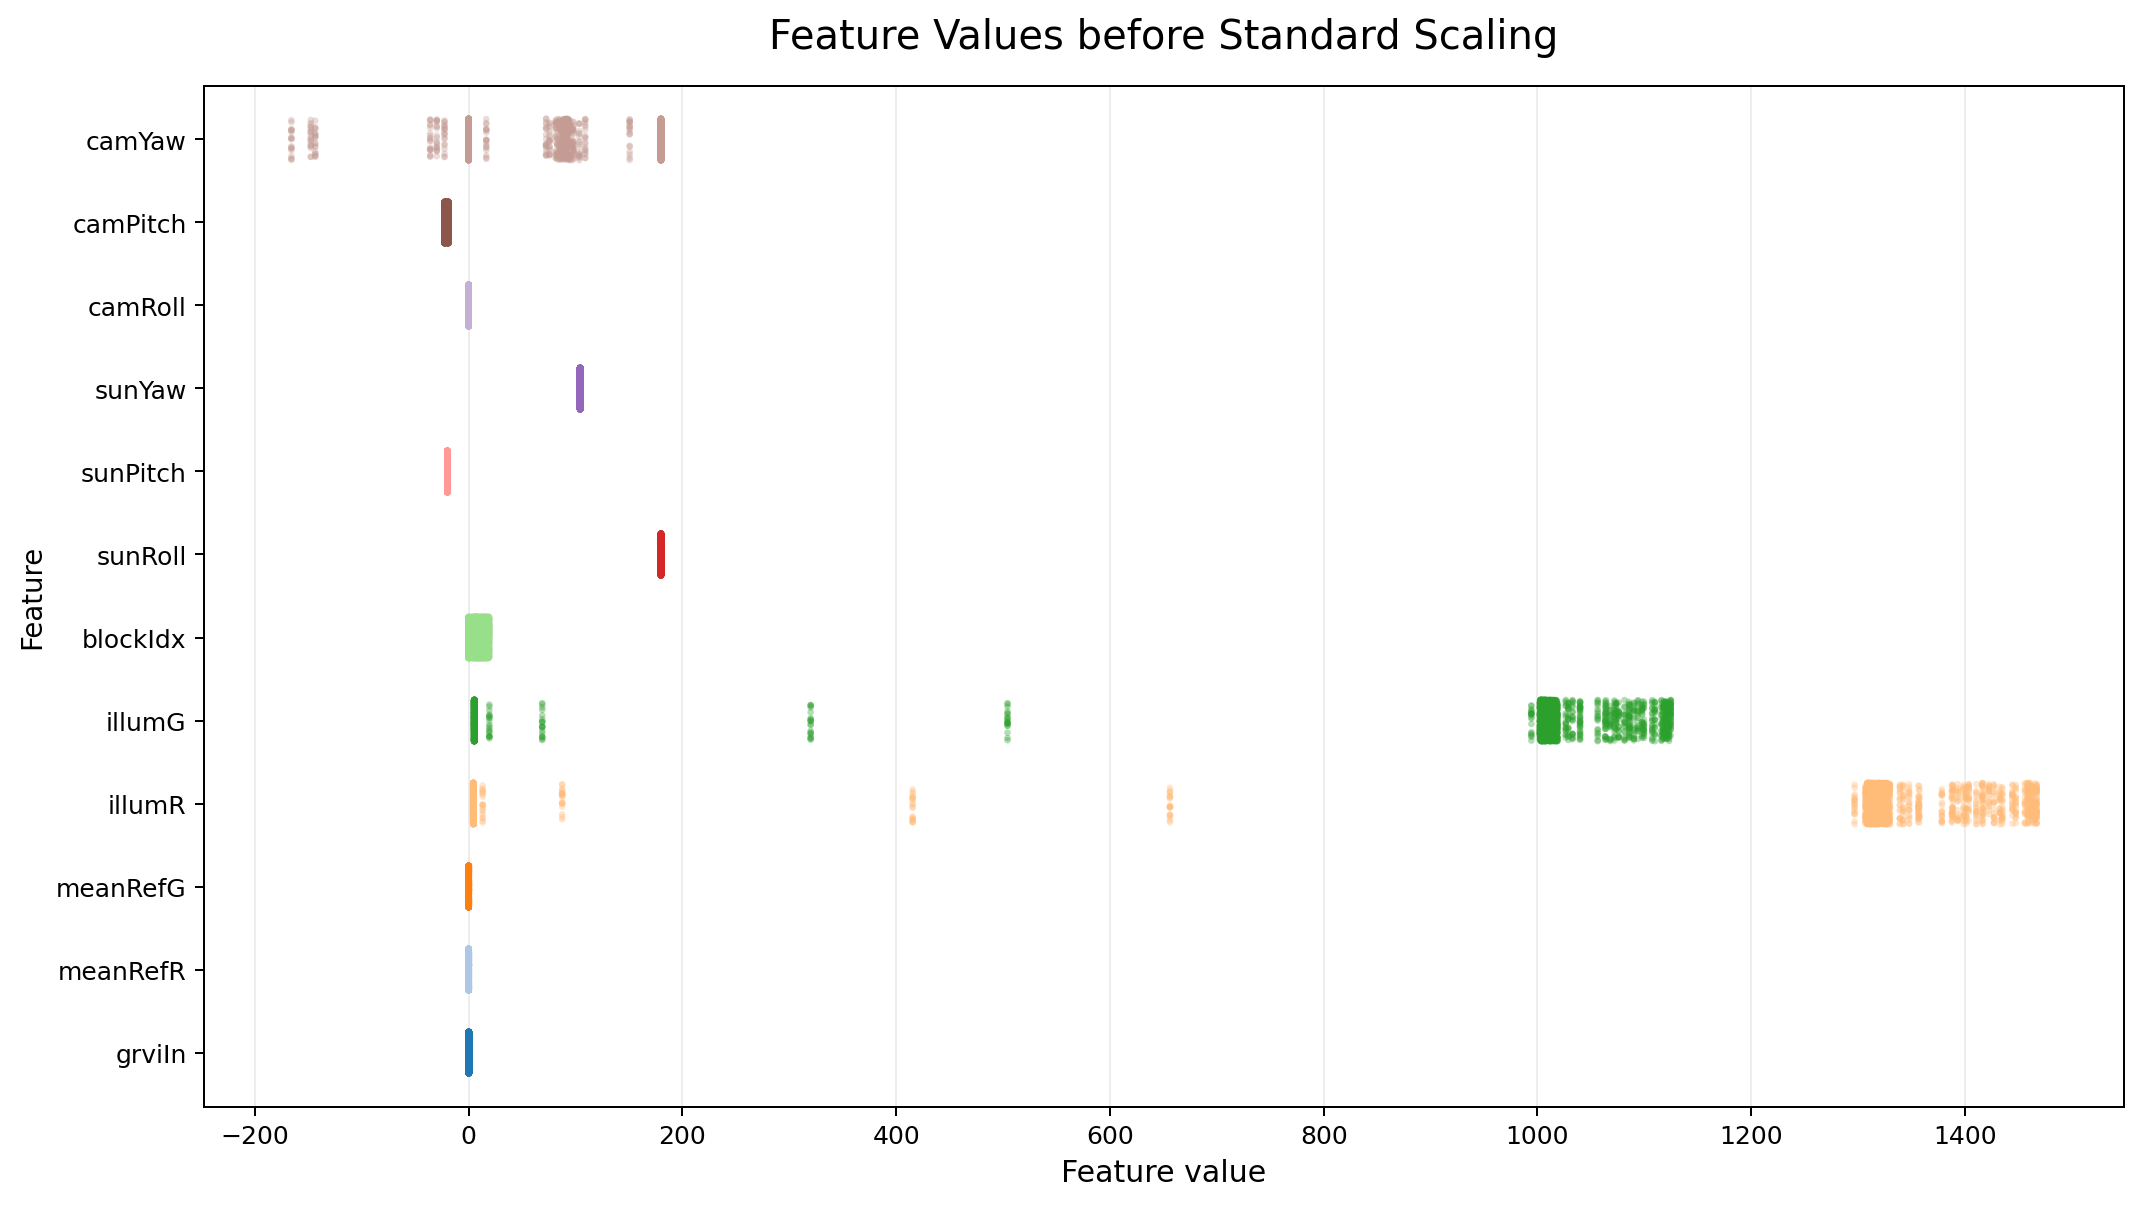
\includegraphics[width=\linewidth]{images/before_standard_scaling.png}
        \caption{Feature values before Standard Scaling}
        \label{ss-before}
    \end{subfigure}\hfill
    \begin{subfigure}{0.48\linewidth}
        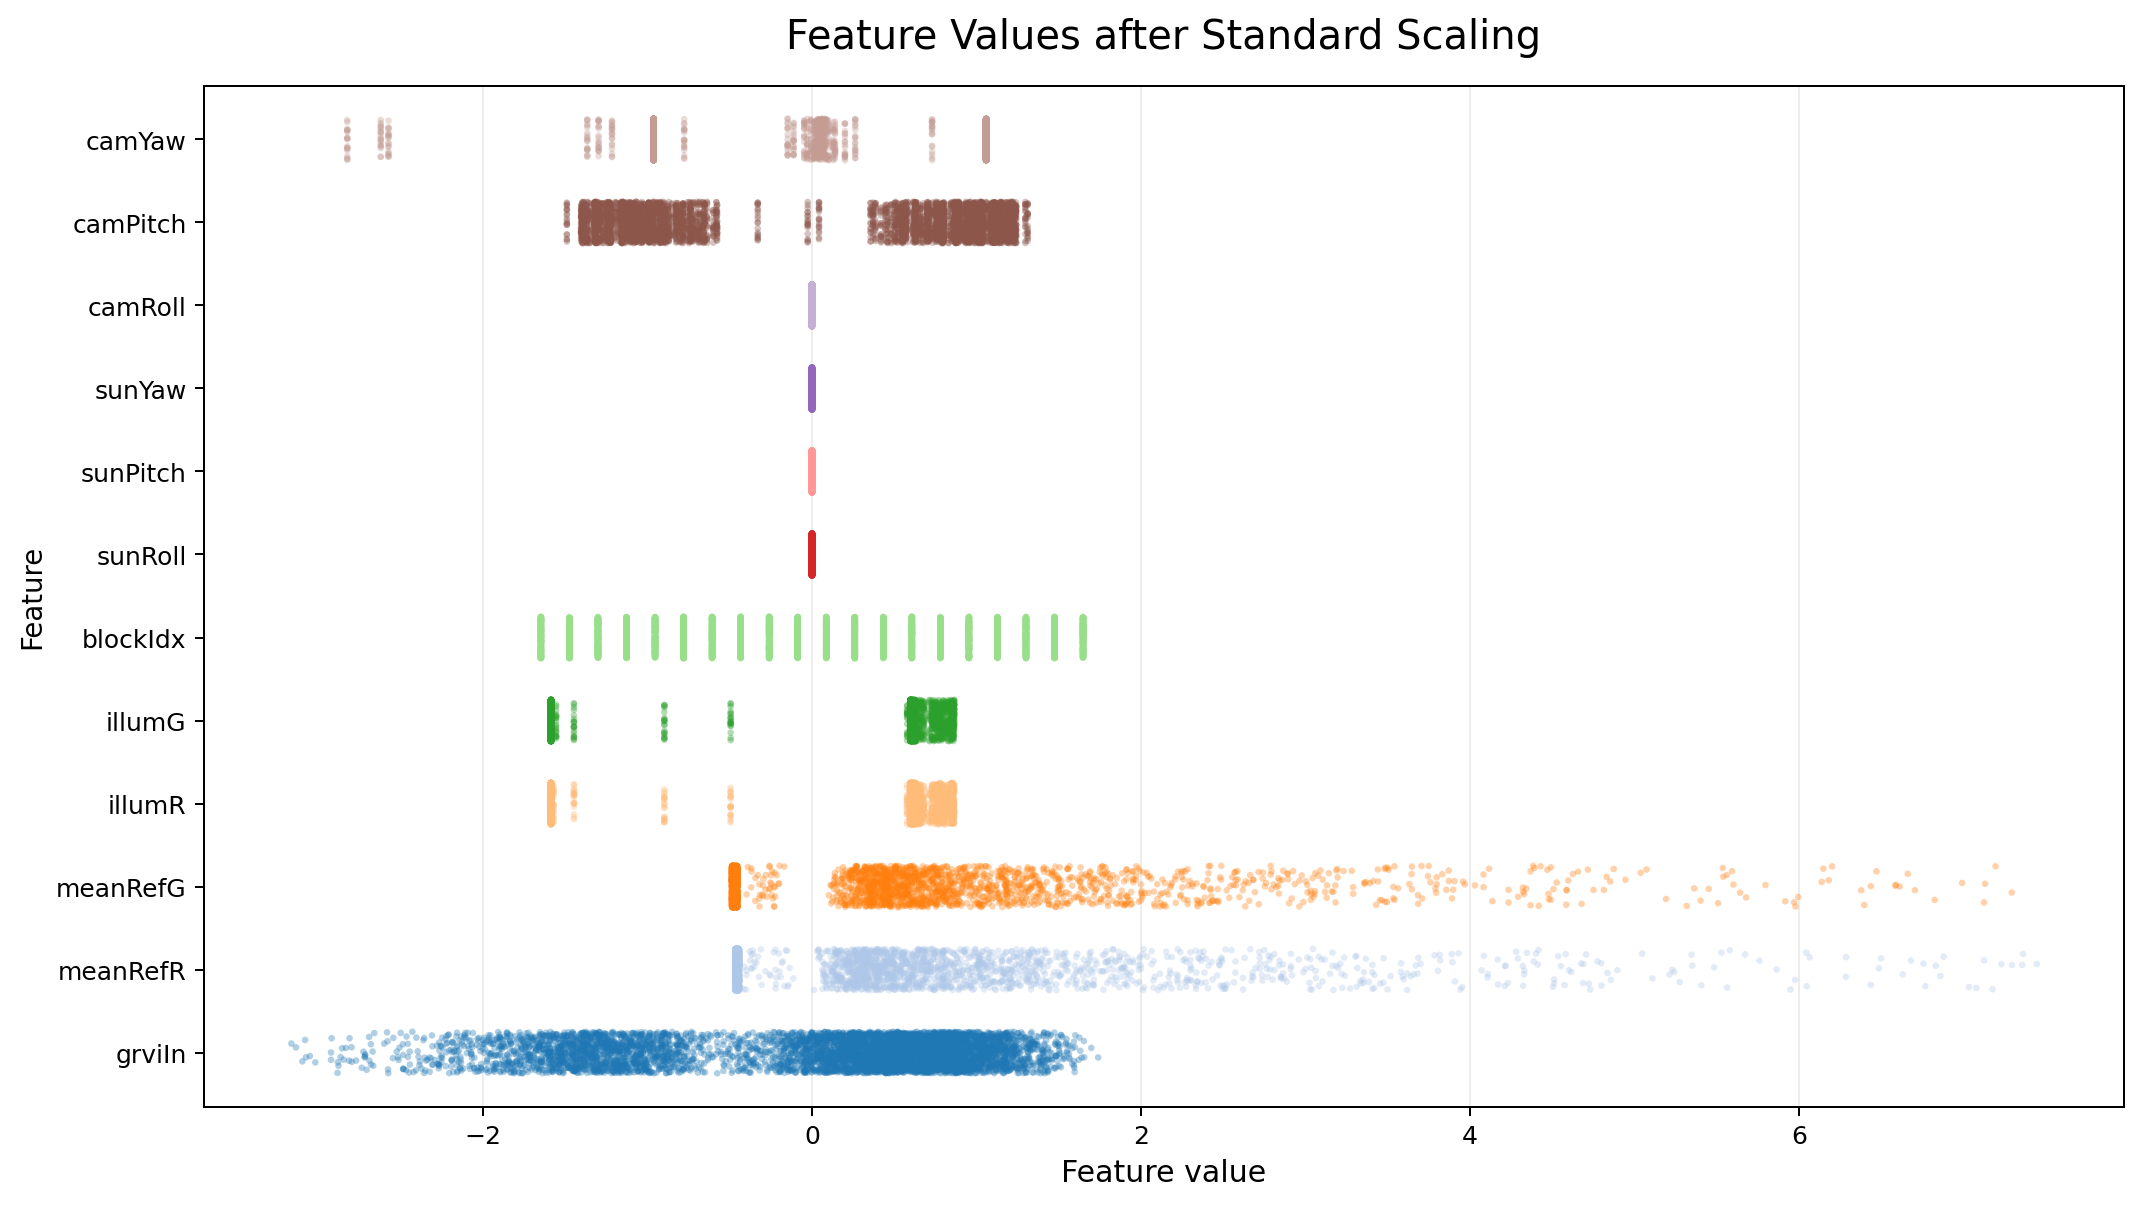
\includegraphics[width=\linewidth]{images/after_standard_scaling.png}
        \caption{Feature values after Standard Scaling}
        \label{ss-after}
    \end{subfigure}
    
    \caption{Scatter plots of the feature values, acquired after a single render sequence. Plot~\ref{ss-before} presents the original feature values, while Plot~\ref{ss-after} shows their standardized counterparts.}
    \label{ss-before-after}
\end{figure}